\documentclass{article}

% Change default font to Helvetica
\usepackage{helvet}
    \renewcommand\familydefault{\sfdefault}
\usepackage[T1]{fontenc}

% Page setup
\usepackage[margin=1in, includefoot, footskip=30pt]{geometry}
\usepackage{setspace}
    \doublespacing%

% Packages
\usepackage{hyperref}
\usepackage{tikz}
    \usetikzlibrary{shapes.geometric}


\title{EDO:\@ A Python library for Evolutionary Dataset Optimisation}
\author{Henry Wilde}

\begin{document}

\maketitle

\section{Summary}

Typically, when faced with a problem in data science, the data is fixed and a
researcher must select an algorithm that is both appropriate for the problem and
performs well on the data. This process is often comprised of a combination of
literature review and then running multiple algorithms on the dataset to choose
a winner based on their objective value. The issue with this process is that it
does not always allow the researcher to consider why certain algorithms perform
better on some datasets and not others, and what makes data ``good'' for their
chosen algorithm.

The purpose of EDO is to allow the user to create populations of artificial
datasets for which a specific algorithm performs well. This is done by passing
the objective function of the algorithm to a genetic algorithm (GA). Therein
each individual represents a particular dataset defined by its dimensions,
values, and the statistical shape of each of its columns. In this way, detailed
information about the individual datasets is retained throughout the algorithm
so that they can be manipulated in a meaningful way, and for the purposes of
analysis once the genetic algorithm has terminated.

EDO has been built in a way that embraces the principles of reproducible
research, and the software itself is tested using a combination of doc, unit and
integration tests with complete coverage. The project is also thoroughly
documented: \href{https://edo.readthedocs.io/}{edo.readthedocs.io}.


\section{The genetic algorithm}

\begin{itemize}
    \item Definitions and walkthrough of each component:
        \begin{itemize}
            \item Individuals
            \item Fitness evaluation
            \item Stopping conditions
            \item Selection
            \item Crossover
            \item Mutation
        \end{itemize}
\end{itemize}

Genetic algorithms form a branch of stochastic optimisation methods encompassed
by more general evolutionary methods. They are characterised by their use of
three biologically inspired operators: selection, crossover and mutation. These
operators form the iterative step in a GA whereby generations of individuals are
improved on over time. A schematic for a general GA is given in
Figure~\ref{fig:flowchart}.

\begin{figure}[htbp]
    \centering%
    \resizebox{0.6\paperwidth}{!}{%
        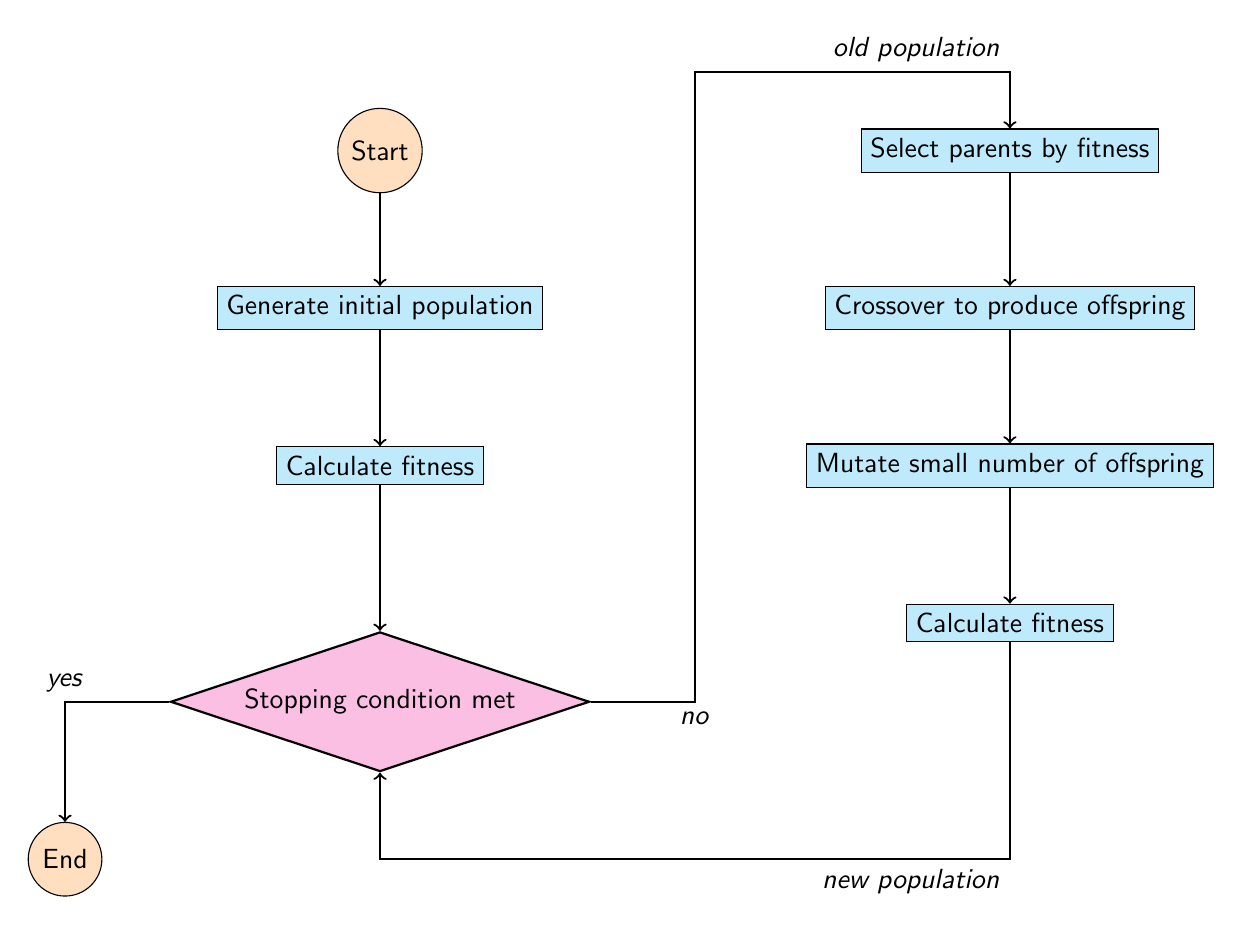
\begin{tikzpicture}
    \node[draw, circle, fill=orange!25] (start) at (0, 0) {Start};
    \node[draw, fill=cyan!25] (initial) at (0, -2) {Generate initial
        population};
    \node[draw, fill=cyan!25] (init-fitness) at (0, -4) {Calculate fitness};
    \node[draw, diamond, thick, aspect=3, fill=magenta!25] (stop) at (0, -7)
        {Stopping condition met};
    \node[draw, circle, fill=orange!25] (end) at (-4, -9) {End};
    \node[draw, fill=cyan!25] (selection) at (8, 0) {Select parents by
        fitness};
    \node[draw, fill=cyan!25] (crossover) at (8, -2) {Crossover to produce
        offspring};
    \node[draw, fill=cyan!25] (mutation) at (8, -4) {Mutate small number of
        offspring};
    \node[draw, fill=cyan!25] (fitness) at (8, -6) {Calculate fitness};

    \draw[->, thick] (start) -- (initial);
    \draw[->, thick] (initial) -- (init-fitness);
    \draw[->, thick] (init-fitness) -- (stop);
    \draw[->, thick] (stop) -- (-4, -7) node[above] {\textit{yes}} -- (end);
    \draw[->, thick] (stop) -- (4, -7) node[below] {\textit{no}} -- (4, 1)
        -- (8, 1) node[above left] {\textit{old population}} -- (selection);
    \draw[->, thick] (selection) to (crossover);
    \draw[->, thick] (crossover) to (mutation);
    \draw[->, thick] (mutation) to (fitness);
    \draw[->, thick] (fitness) -- (8, -9) node[below left] {\textit{new
        population}} -- (0, -9) -- (stop);
\end{tikzpicture}

    }
    \caption{A generic genetic algorithm}%
    \label{fig:flowchart}
\end{figure}



\section{Examples}

\begin{itemize}
    \item Take the ``optimise \(x^2\)'' example from the docs
    \item Use a more complicated example wrt.\ the fitness landscape
\end{itemize}

\section{Limitations}

\begin{itemize}
    \item Scaling issues with complexity
    \item Not following `building block principle'
    \item Distributions are unreliable for small datasets
\end{itemize}

\end{document}
